% \usemintedstyle[julia]{native}

Реализация вышеобозначенных разностных схем производилась с помощью языка программирования \texttt{Julia}\cite{bezanson2017julia}. 

В качестве иллюстрации простоты явной разностной схемы, в листинге \ref{listing:explicit_scheme} приведена её реализация для одномерного линейного уравнения теплопроводности.
\begin{listing}
    \begin{minted}[
        frame=lines,
        framesep=2mm,
        fontsize=\footnotesize,
        linenos=true,
        autogobble
        ]{julia}
    function explicit_scheme(f, u0, mu1, mu2, T, Nx, Nt)
        x = range(0, 1, length = Nx) # Точки секти по оси `x`
        t = range(0, T, length = Nt) # Точки сетки по оси `t`
        c = step(t) / step(x)^2 # Коэффициент Куранта
    
        u = zeros(Nx, Nt) # Матрица, хранящая решение разностной задачи
    
        u[:, 1] .= u0.(x) # Учёт начальных условий
        u[1, :] .= mu1.(t) # Учёт граничных условий на левом конце
        u[end, :] .= mu2.(t) # Учёт граничных условий на правом конце
    
        for j in 1:(Nt - 1) # Цикл по всем слоям
            for i in 2:(Nx - 1)
                u[i, j + 1] = u[i, j] + c * (u[i + 1, j] - 2 * u[i, j] + u[i - 1, j]) + 
                f(x[i], t[j])
            end
        end
    
        return u
    end
    \end{minted}
    \caption{Реализация явной схемы для уравнения $u_t = u_{xx} + f$}
    \label{listing:explicit_scheme}
\end{listing}
Заметим, что схема реализована для уравнения $u_t = u_{xx} + f$ на отрезке $x \in [0, 1]$, поскольку более общий вид уравнения $u_t = a^2 u_{xx} + \tilde{f}$ на отрезке $[a, b]$ сводится к первому линейной заменой $ t \mapsto \tilde{t} = \frac{(b - a)^2}{a^2} t, \quad x \mapsto \tilde{x} = \frac{x - a}{b - a}$.
Работоспособность программы была проверена на некоторых тестовых задачах \cite{горюнов2015методы}.
Так, для задачи
\begin{equation}\label{eq:task_1}
    \begin{cases}
        u_t = u_{xx} + f, & (x, t) \in (0, 1) \times (0, T]\\
        u(x, 0) = x\sin (3\pi x), & x \in [0, 1]\\
        \begin{aligned}
            & \textstyle u(0, t) = 0\\
            & \textstyle u(1, t) = 0
        \end{aligned}, & t \in [0, T]
    \end{cases}
\end{equation}
расчитано решение для $T = 0.05$ для различного набора сеток с числом точек по оси времени $N_t = 25001$ и числом точек по оси $x$ в пределах от $N_x = 10$ до $N_x = 500$.
Заметим, что выбор такого, казалось бы, необоснованно большого числа точек по оси времени диктуется неустойчивостью явной разностной схемы: из условия устойчивости $\frac{\Delta t}{(\Delta x)^2} < \frac{1}{2}$ следует, что для $N_x = 500$ требуется $N_t > 25000$.
В таких простых, тестовых задачах такое соотношение ещё приемлемо, и современные компьютеры позволяют получить ршение достаточно быстро.
Однако в более сложных, многомерных задачах с резкими неоднородностями, требующими достаточно мелкого пространственного шага, это условие становится трудно выплонимым (такая точность по оси времени просто не требуется).
Явная схема была реализована только для линейного уравнения.
Как уже отмечалось выше, применения явной схемы нецелесообразно для квазилинейных уравнений.



\begin{figure}
    \centering
    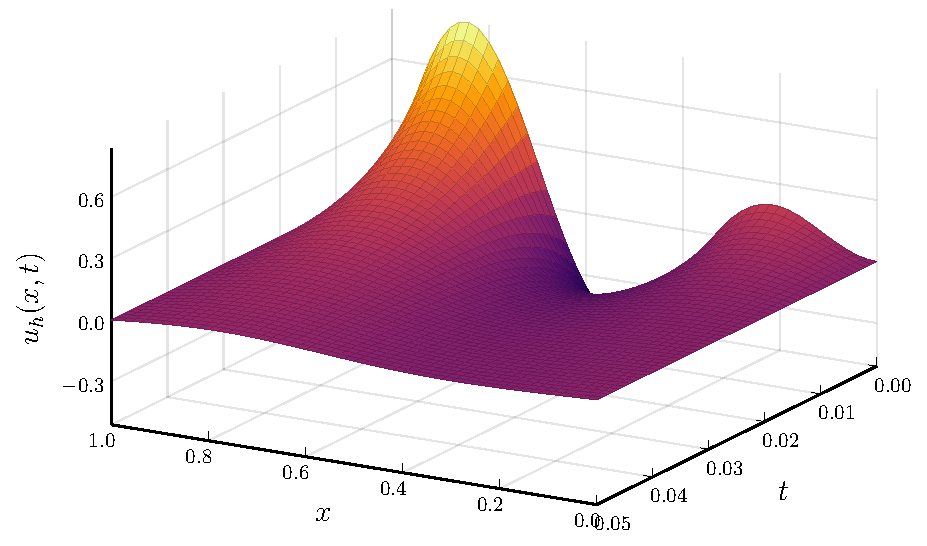
\includegraphics{Разностные_схемы_на_статических_сетках/Программный_код_примеры_расчётов/explicit_scheme/problem_1_explicit_surface.pdf}
    \caption{Численное решение задачи \eqref{eq:task_1} для $N_x = 500$ и $N_t = 25\,000$}
    \label{fig:problem_1_explicit_surface}
\end{figure}
\begin{figure}
    \centering
    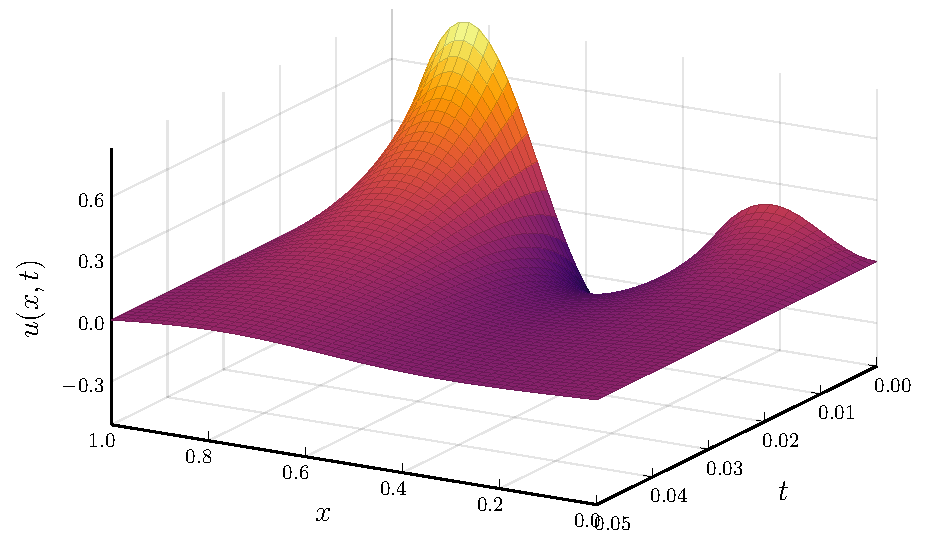
\includegraphics{Разностные_схемы_на_статических_сетках/Программный_код_примеры_расчётов/explicit_scheme/problem_1_analytic_surface.pdf}
    \caption{Аналитическое решение задачи \eqref{eq:task_1}}
    \label{fig:problem_1_analytic_surface}
\end{figure}
\begin{figure}
    \centering
    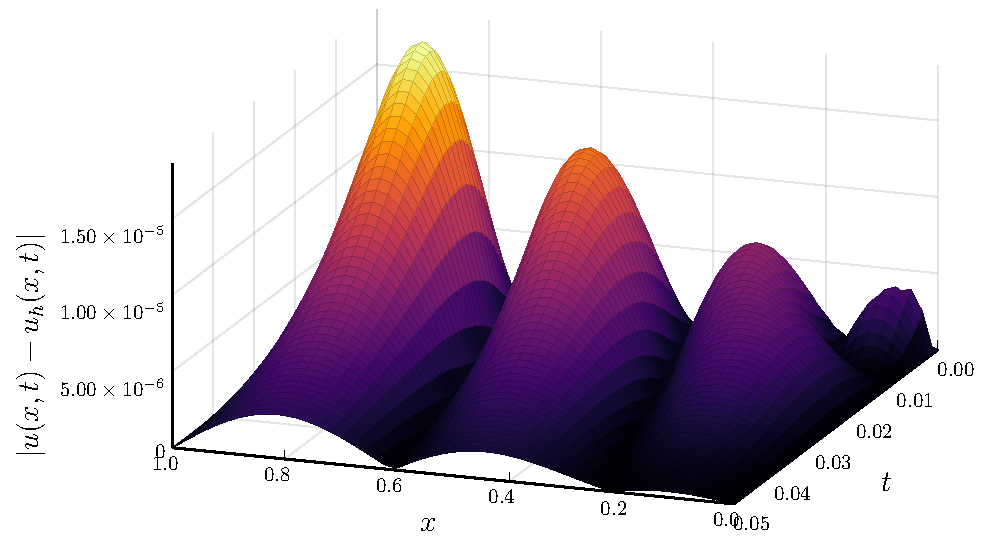
\includegraphics{Разностные_схемы_на_статических_сетках/Программный_код_примеры_расчётов/explicit_scheme/problem_1_explicit_error_surface.pdf}
    \caption{График локальной ошибки численного решения задачи \eqref{eq:task_1}}
    \label{fig:problem_1_explicit_error_surface}
\end{figure}
\begin{figure}
    \centering
    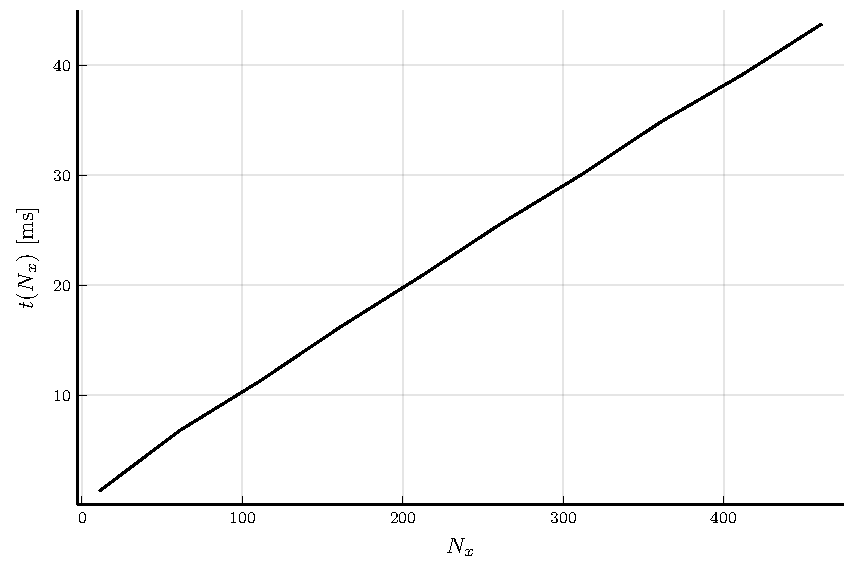
\includegraphics{Разностные_схемы_на_статических_сетках/Программный_код_примеры_расчётов/explicit_scheme/problem_1_explicit_time.pdf}
    \caption{График зависимости времени счёта от числа точек сетки $t(N_x)$ (в мс).}
    \label{fig:problem_1_explicit_time}
\end{figure}
На \figref{fig:problem_1_explicit_surface} представлено численное решение задачи как поверхность-график $u_h(x, t)$, полученное явной схемой для $N_x = 500$ и $N_t = 25000$.
На \figref{fig:problem_1_analytic_surface} представлен график зависимости аналитического решения задачи, полученного методом разделения переменных Фурье:
\begin{equation*}
    u(x, t) = \frac{1}{2}e^{-(3\pi)^2 t}\sin (3\pi x) - \frac{48}{\pi^2}\sum\limits_{m=1}^{\infty} \frac{m}{(9 - 4m^2)^2}e^{-(2\pi m)^2 t}\sin (2\pi m x)
\end{equation*}
Для точного сравнения также на \figref{fig:problem_1_explicit_error_surface} представлен график зависимости локальной ошибки $|u(x, t) - u_h(x, t)|$.
Видно, что в случае линейного уравнения без особенностей решения погрешность численного решения в среднем \glqq размазана\grqq по всей области.

Для проверки утверждения о скорости счёта разностной схемы также построен график зависимости среднего времени выполнения программы (как среднее время от $\sim 100-200$ запусков программы для одних и тех же входных данных) как функции от числа точек сетки по оси $x$ (\seefigref{fig:problem_1_explicit_time}).





Реализация неявной схемы требует написания алгоритма прогонки для решения систем линейных уравнений с трёхдиагональной матрицей.
В листинге \ref{listing:tridiagonal_algorithm} представлен код алгоритма прогонки.
\begin{listing}
    \begin{minted}[
        frame=lines,
        framesep=2mm,
        fontsize=\footnotesize,
        linenos,
        autogobble
        ]{julia}
    # Оптимальный по памяти алгоритм прогонки в случае, если его нужно запускать много раз
    function tridiagonal_algorithm!(
            a::Vector{<:T}, b::Vector{<:T}, x::Vector{<:T},
            A::Vector{<:T}, B::Vector{<:T}, C::Vector{<:T}, D::Vector{<:T}
        ) where {T <: Number}
    
        a[1] = - C[1] / B[1]
        b[1] = D[1] / B[1]
        for i=2:(length(B)-1)
            a[i] = - C[i] / (B[i] + A[i-1] * a[i-1])
            b[i] = (D[i] - A[i-1] * b[i-1]) / (B[i] + A[i-1] * a[i-1])
        end
        b[end] = (D[end] - A[end] * b[end-1]) / (B[end] + A[end] * a[end-1])
    
        # обратный ход
        x[end] = b[end]
        for i = length(B)-1:-1:1
            x[i] = a[i]*x[i+1] + b[i]
        end
    end
    \end{minted}
    \caption{Реализация алгоритма прогонки}
    \label{listing:tridiagonal_algorithm}
\end{listing}
Дополнительные переменные $\alpha, \beta, x$ передаются в функцию \texttt{tridiagonal\_algorithm} с целью экономии памяти.
Решение уравнения теплопроводности требует многократного выполнения алгоритма прогонки, поэтому общие временные переменные выделяются отдельно и сокращают количество ненужных аллокаций.
В листинге \ref{listing:implicit_scheme} приведена реализация неявной схемы для одномерного квазилинейного уравнения теплопроводности.
\begin{listing}
    \begin{minted}[
        frame=lines,
        framesep=2mm,
        fontsize=\footnotesize,
        linenos,
        autogobble
        ]{julia}
    function implicit_scheme(k, f, u0, mu1, mu2, T, Nx, Nt)
        x = range(0, 1, length = Nx) # Точки секти по оси `x`
        dx = step(x)
        t = range(0, T, length = Nt) # Точки сетки по оси `t`
        dt = step(t)
    
        u = zeros(Nx, Nt) # Матрица, хранящая решение разностной задачи
        u[:, 1] .= u0.(x) # Учёт начальных условий
        u[1, :] .= mu1.(t) # Учёт граничных условий на левом конце
        u[end, :] .= mu2.(t) # Учёт граничных условий на правом конце
    
        # Временные переменные для алгоритма прогонки
        A, C = (zeros(Nx) for i in 1:2)
        B, D, a, b, xt = (zeros(Nx) for i in 1:5)
        B[1] = B[end] = 1
        C[1] = A[end] = 0
    
        for j in 1:(Nt - 1) # Цикл по временным слоям
            # Обновление коэффициентов тридиагональной матрицы
            D[1] = u[1, j + 1]
            D[end] = u[end, j + 1]
            for i = 2:(Nx - 1)
                A[i - 1] = -dt * k(0.5 * (u[i - 1, j] + u[i, j]))
                B[i] = dx^2 + dt * (
                    k(0.5 * (u[i, j] + u[i + 1, j])) +
                    k(0.5 * (u[i - 1, j] + u[i, j]))
                )
                C[i] = -dt * k(0.5 * (u[i, j] + u[i + 1, j]))
                D[i] = dx^2 * u[i, j] + dt * dx^2 * f(x[i], t[j])
            end
            tridiagonal_algorithm!(a, b, xt, A, B, C, D) # Метод прогонки
            u[:, j + 1] .= xt
        end
    
        return u
    end
    \end{minted}
    \caption{Реализация неявной схемы для уравнения $u_t = (ku_x)_x + f$}
    \label{listing:implicit_scheme}
\end{listing}
Работоспособность программы проверена на тех же тестовых задачах, что и для явной схемы.
\begin{figure}
    \centering
    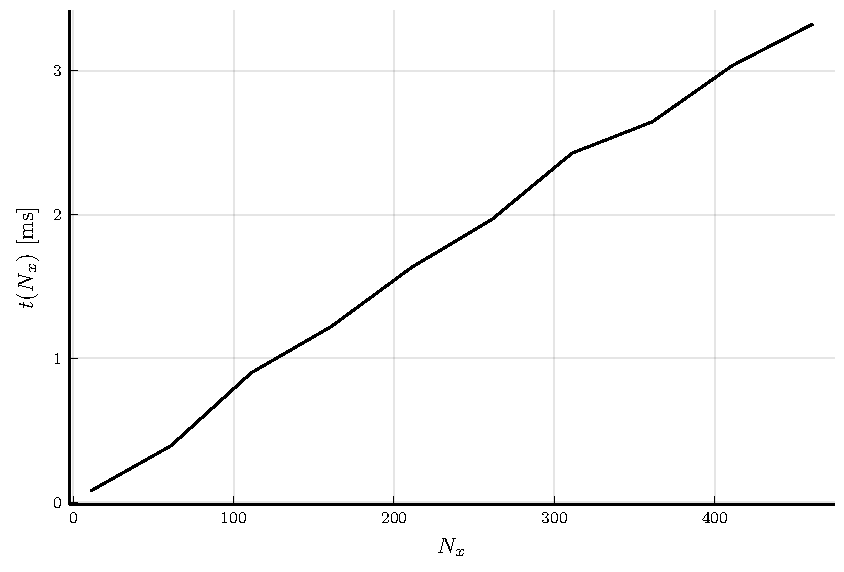
\includegraphics{Разностные_схемы_на_статических_сетках/Программный_код_примеры_расчётов/explicit_scheme/problem_1_implicit_time.pdf}
    \caption{График зависимости времени счёта от числа точек сетки для неявной схемы}
    \label{fig:problem_1_implicit_time}
\end{figure}
Из рисунка \ref{fig:problem_1_implicit_time} видно, что, хоть абсолютная скорость счёта неявной схемы и уступает явной, асимптотика (то есть линейная зависимость) остаётся точно такой же.


Для проверки правильности учёта квазилинейности уравнения программа проверена на задаче, рассмотренной в статье~\cite{самарский1963примеры}:
\begin{equation*}
    \left\{
        \begin{aligned}
            &\frac{\partial u}{\partial t} = \frac{\partial }{\partial x}\left( \frac{1}{2}u^2 \frac{\partial u}{\partial x} \right), && (x, t) \in (0, 1)\times(0.1, 0.4)\\
            &\begin{aligned}
            &u(0, t) = 10\sqrt{t}\\
            &u(1, t) = 0
            \end{aligned}, && t\in [0.1, 0.4]\\
            &u(x, 0.1) = \left\{ \begin{aligned}
                &2\sqrt{5(0.5 - x)}, && x \le 0.5\\
                & 0, && x\ge 0.5
            \end{aligned}\right. , && x \in [0, 1]
        \end{aligned}
    \right.
\end{equation*}
\begin{figure}
    \centering
    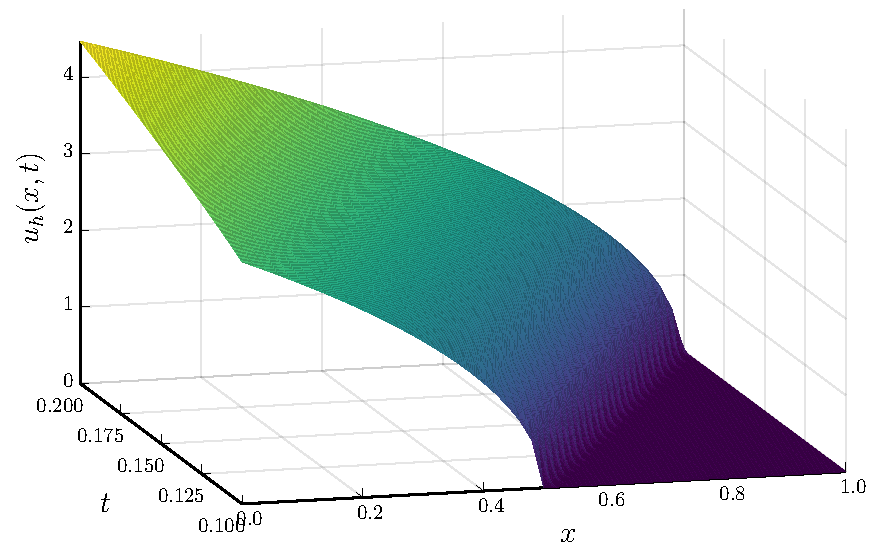
\includegraphics{Разностные_схемы_на_статических_сетках/Программный_код_примеры_расчётов/explicit_scheme/problem_2_implicit_surface.pdf}
    \caption{Численное решение задачи \eqref{eq:problem_2} с параметрами сетки $N_x = 50$, $N_t = 500$}
    \label{fig:problem_2_implicit_surface}
\end{figure}
\begin{figure}
    \centering
    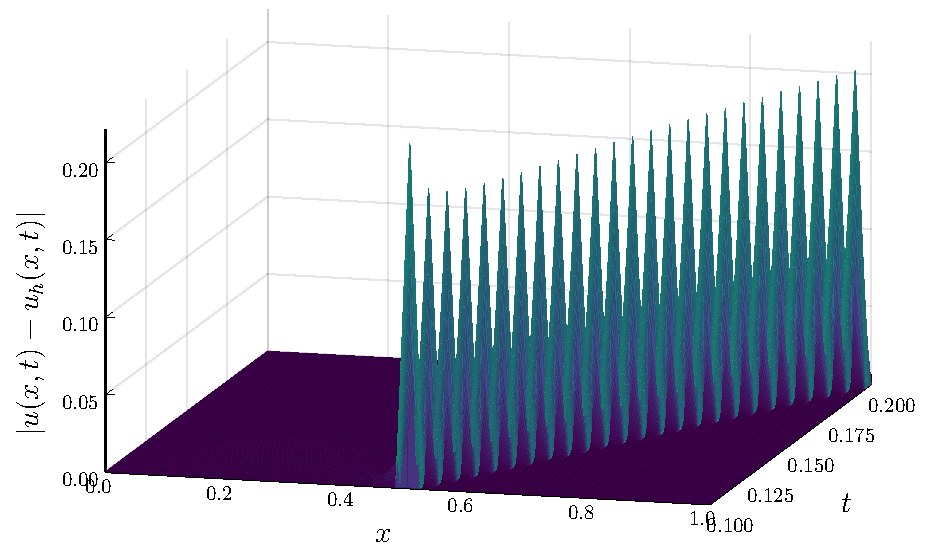
\includegraphics[width=\textwidth]{Разностные_схемы_на_статических_сетках/Программный_код_примеры_расчётов/explicit_scheme/problem_2_implicit_error_surface.pdf}
    \caption{График локальной ошибки численного решения}
    \label{fig:problem_2_implicit_error_surface}
\end{figure}
\begin{figure}
    \centering
    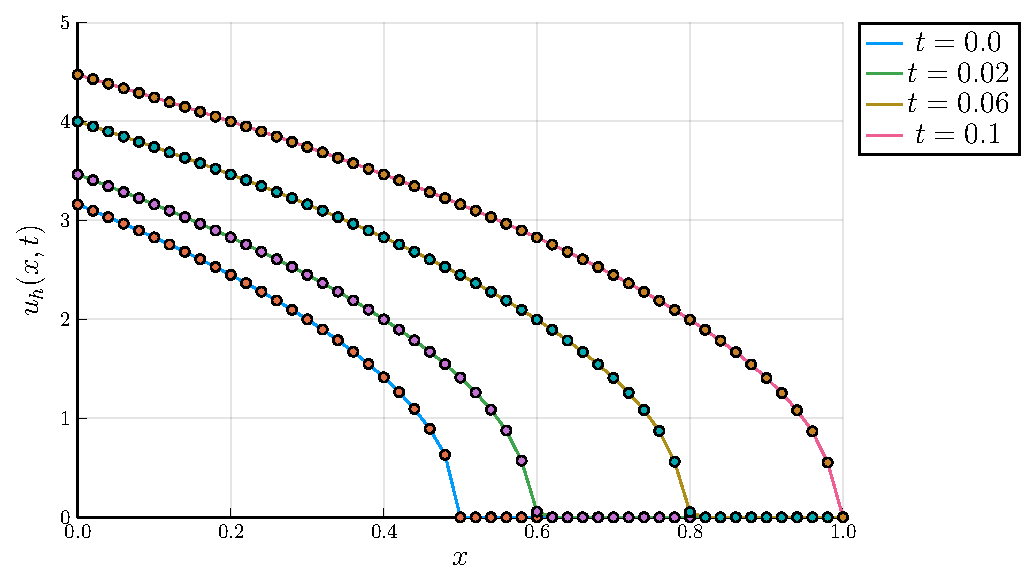
\includegraphics{Разностные_схемы_на_статических_сетках/Программный_код_примеры_расчётов/explicit_scheme/problem_2_implicit_Samarski.pdf}
    \caption{Профили волны в некоторые моменты времени}
    \label{fig:problem_2_implicit_Samarski}
\end{figure}
\begin{figure}
    \centering
    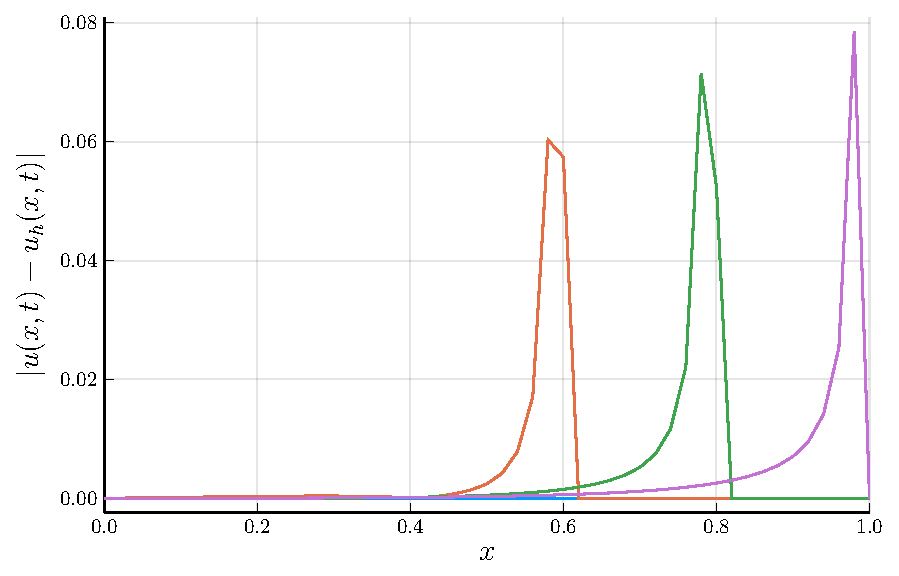
\includegraphics{Разностные_схемы_на_статических_сетках/Программный_код_примеры_расчётов/explicit_scheme/problem_2_implicit_error_Samarski.pdf}
    \caption{Графики локальных погрешностей для некоторых моментов времени.}
    \label{fig:problem_2_implicit_error_Samarski}
\end{figure}
\begin{figure}
    \centering
    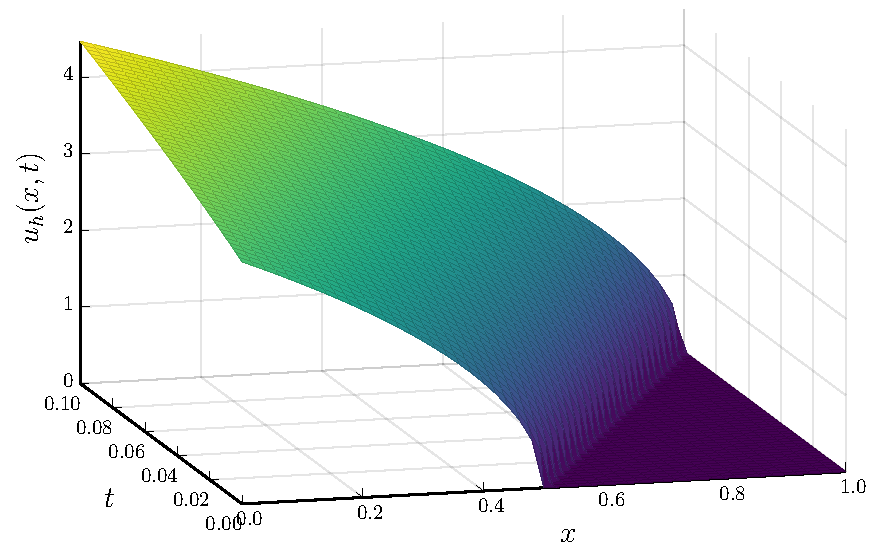
\includegraphics{Разностные_схемы_на_статических_сетках/Программный_код_примеры_расчётов/explicit_scheme/problem_2_implicit_surface_high.pdf}
    \caption{Более точное решение задачи \eqref{eq:problem_2}, полученное для параметров сетки $N_x = 5000$, $N_t = 5000$.}
    \label{fig:problem_2_implicit_surface_high}
\end{figure}
\begin{figure}
    \centering
    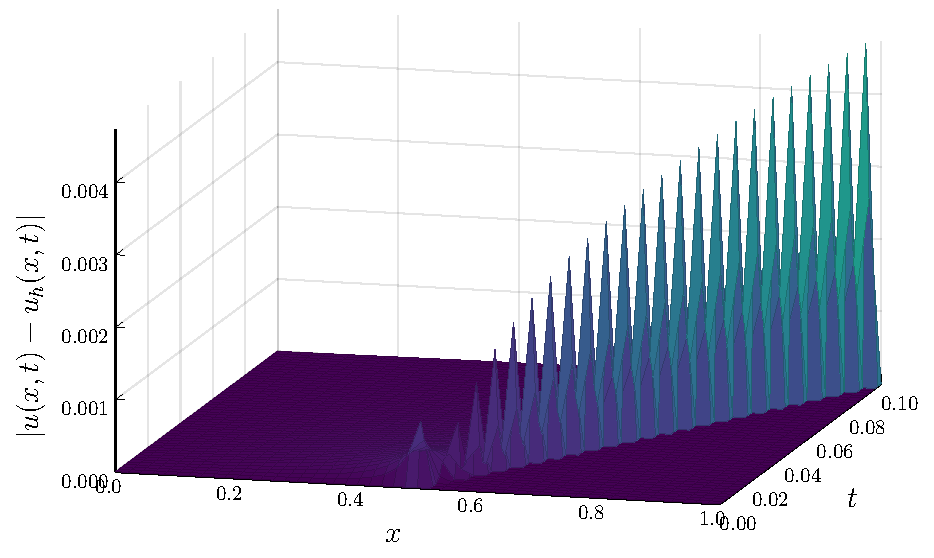
\includegraphics{Разностные_схемы_на_статических_сетках/Программный_код_примеры_расчётов/explicit_scheme/problem_2_implicit_error_surface_high.pdf}
    \caption{График локальной погрешности, полученный для параметров сетки $N_x = 5000$, $N_t = 5000$. Видно, что относительно все ошибки сосредоточены в окрестности фронта волны.}
    \label{fig:problem_2_implicit_error_surface_high}
\end{figure}
На \figref{fig:problem_2_implicit_surface} приведено численное решение, полученное неявной схемой на сетке с $N_x = 50$, $N_t = 50$.
Также на \figref{fig:problem_2_implicit_error_surface} представлен график зависимости локальной ошибки, посчитанной с помощью аналитического решения:
\begin{equation}\label{eq:problem_2}
    u(x, t) = \left\{
        \begin{aligned}
            &\left[ \sigma c\varkappa_0^{-1} (ct + x_1 - x) \right]^{1/\sigma}, && x \le x_1 + ct\\
            &0, && x \ge x_1 + ct
        \end{aligned}
    \right.
\end{equation}
где $\sigma = 2$, $\varkappa_0 = 0.5$, $x_1 = 0$, $c = 5$. 
Для большей наглядности представлены также два одномерных графика, показывающие профиль решения и локальную погрешность в некоторые моменты времени (\seefigref{fig:problem_2_implicit_Samarski} и \figref{fig:problem_2_implicit_error_Samarski})

Видно, что основная погрешность сосредоточена в точках \emph{температурного фронта волны}: всюду, кроме некоторых точек около фронта, в которых производные решения терпят разрыв, отклонение приближённого решения от аналитического не превосходит $2\cdot 10^{-3}$.
Для достижения такой же точности и в \emph{вблизи особых точек} решения необходима достаточно мелкая сетка.
Были выбраны параметры $N_x = 5000$, $N_t = 5000$, график численного решения приведён на \figref{fig:problem_2_implicit_surface_high}.
Однако из \figref{fig:problem_2_implicit_error_surface_high} видно, что даже с настолько мелкой сеткой ошибки в близи особых точек решения остаются весьма заметными.
Более того, решение во всей остальной области оказывается \emph{на порядки} точнее решения вблизи особых точек.
Дальнейшее измельчение сетки будет приводить к огромным, бесполезным расчётным затратам.

Данный пример хорошо демонстрирует причину возникновения метода локально-адаптивных сеток.
В одномерном случае с одной особой точкой эта ситуация может показаться не столь плохой.
Для многомерных же задач с большим числом особенностей и сильно меняющимися масштабами решения, где для получения заданной точности приходится использовать минимально необходимый шаг сетки во всей области сразу, число ненужных операций алгоритма значительно возрастает до недопустимых значений. 

Как уже отмечалась, в задачах с размерностью $p > 1$ получающиеся в неявной схеме системы не будут трёхдиагональными, однако по-прежнему останутся достаточно разреженными.
Реализация такой схемы заключается в прямом создании матрицы системы на каждом временном слое и решении с помощью общего алгоритма исключения переменных Гаусса.

\begin{listing}
    \begin{minted}[
        frame=lines,
        framesep=2mm,
        fontsize=\footnotesize,
        linenos=true,
        autogobble,
        mathescape
        ]{julia}
    function local_scheme(
        k1, k2, f,
        u0, mu_1, mu1, mu_2, mu2,
        Lx, Ly, T, Nx, Ny, Nt
        )
    
        # Создание сетки
        x = range(0, Lx, length = Nx); dx = step(x)
        y = range(0, Ly, length = Ny); dy = step(y)
        t = range(0, T, length = Nt);  dt = step(t)
    
        u = zeros(Nx, Ny, Nt) # Массив, хранящий решение

        # Временные переменные для прогонки
        A, C = (Tuple(zeros(N - 1) for N in [Nx Ny]) for i in 1:2)
        B, D, a, b, xt = (Tuple(zeros(N) for N in [Nx Ny]) for i in 1:5)
        B[1][1] = B[1][end] = B[2][1] = B[2][end] = 1
        C[1][1] = C[2][1] = A[1][end] = A[2][end] = 0
        w = zeros(Nx, Ny)

        for i in 1:Nx, j in 1:Ny u[i, j, 1] = u0(x[i], y[j]) end # н.у.
        for j in 1:(Nt - 1) # Цикл по временным слоям
            for k in 1:Ny # Сначала решаем задачу вдоль оси $x$ для всех $y_k$
                for i in 2:(Nx - 1) # Создание трёхдиагональной матрицы
                    A[1][i - 1] = -k1(0.5 * (u[i - 1, k, j] + u[i, k, j])) / dx^2
                    B[1][i] = 1/dt + (
                        k1(0.5 * (u[i - 1, k, j] + u[i, k, j])) +
                        k1(0.5 * (u[i + 1, k, j] + u[i, k, j]))
                    ) / dx^2
                    C[1][i] = -k1(0.5 * (u[i + 1, k, j] + u[i, k, j])) / dx^2
                    D[1][i] = u[i, k, j] / dt + 0.5 * f(x[i], y[k], t[j] + 0.5 * dt)
                end
                D[1][1] = mu_1(y[k], t[j] + 0.5 * dt); D[1][end] = mu1(y[k], t[j] + 0.5 * dt)
                tridiagonal_algorithm!(a[1], b[1], xt[1], A[1], B[1], C[1], D[1])
                w[:, k] .= xt[1]
            end
            for i in 1:Nx # Теперь решаем задачу вдоль оси $y$ для всех $x_i$
                for k in 2:(Ny - 1) # Вся суть далее та же самая
                    A[2][k - 1] = -k2(0.5 * (w[i, k] + w[i, k - 1])) / dy^2
                    B[2][k] = 1/dt + (
                        k2(0.5 * (w[i, k] + w[i, k - 1])) +
                        k2(0.5 * (w[i, k + 1] + w[i, k]))
                    ) / dy^2
                    C[2][k] = -k2(0.5 * (w[i, k] + w[i, k + 1])) / dy^2
                    D[2][k] = w[i, k] / dt + 0.5 * f(x[i], y[k], t[j + 1])
                end
                D[2][1] = mu_2(x[i], t[j + 1]); D[2][end] = mu2(x[i], t[j + 1])
                tridiagonal_algorithm!(a[2], b[2], xt[2], A[2], B[2], C[2], D[2])
                u[i, :, j + 1] .= xt[2]
            end
        end
        return u
    end
    \end{minted}
    \caption{Локально-одномерная схема для двумерного уравнения теплопроводности $u_t = (k_1u_x)_x + (k_2 u_y)_y + f$}
    \label{listing:loc_scheme}
\end{listing}
Локально-одномерная схема в сущности решает $N^{p - 1}$ одномерных задач, поэтому её реализация похожа на неявную схему, но с некоторыми отличиями.
В листинге \ref{listing:loc_scheme} приведёт код этой схемы для двумерного квазилинейного уравнения теплопроводности (на случай больших размерностей код модифицируется очевидным образом).

\begin{figure}
    \centering
    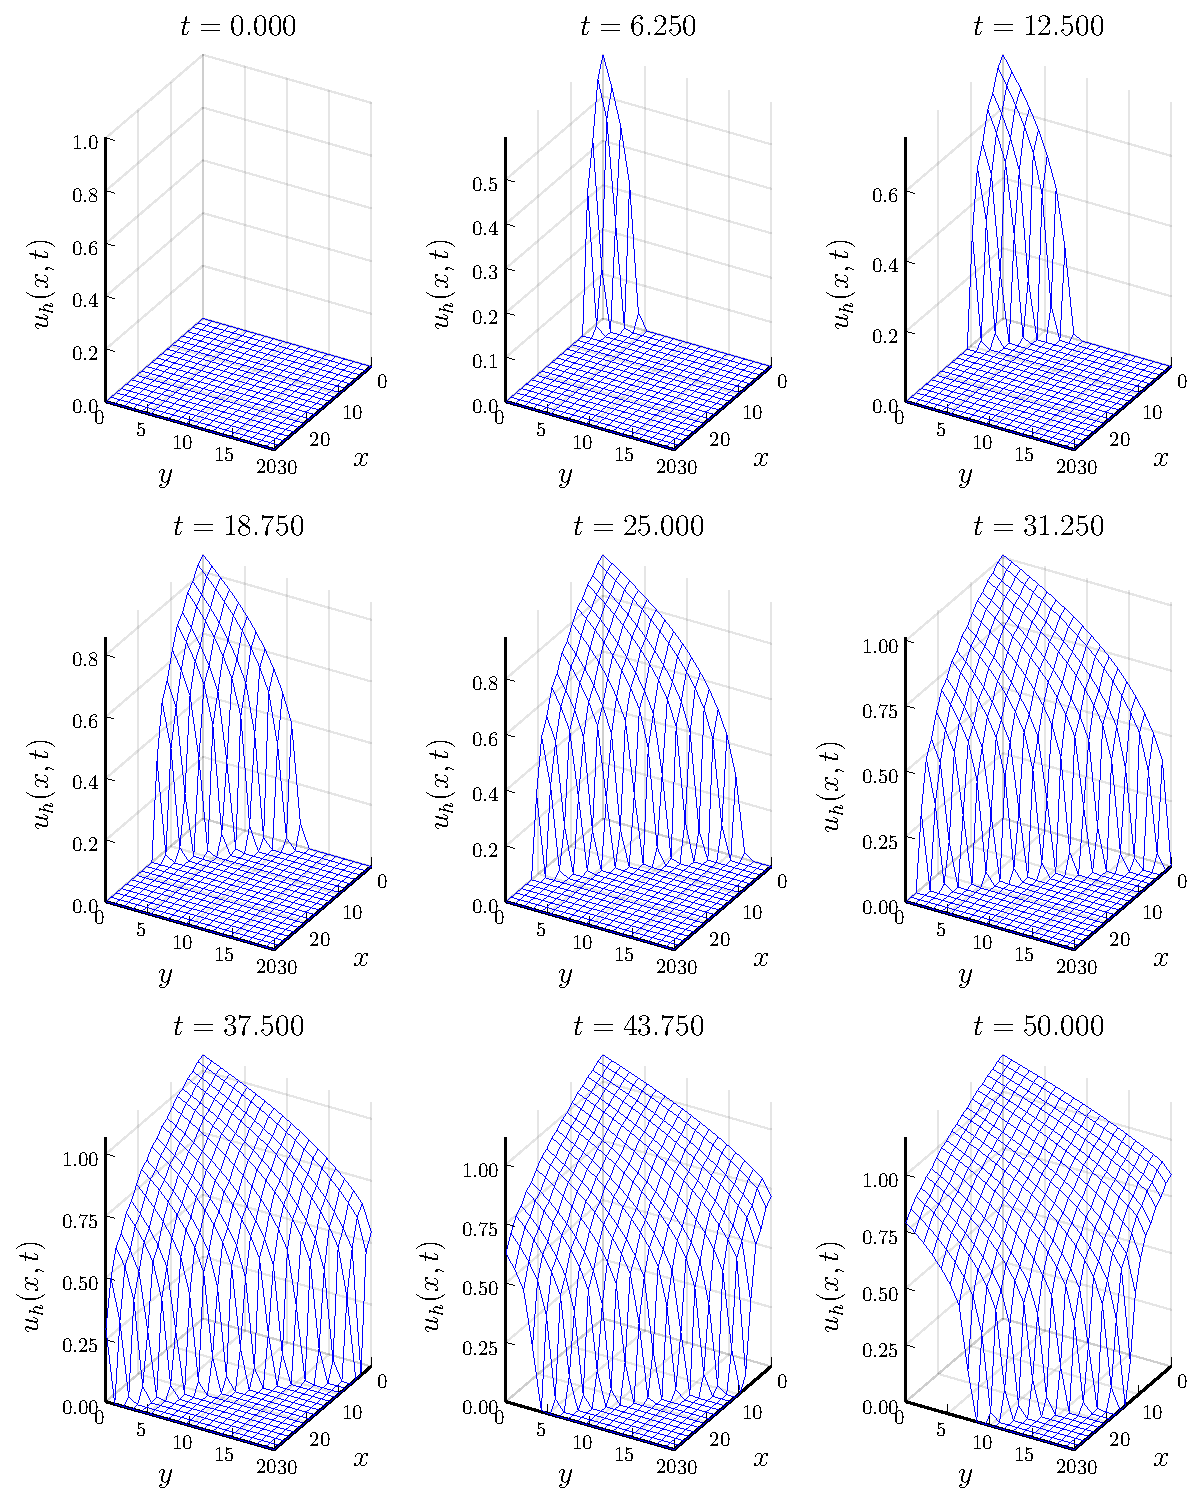
\includegraphics[width=\textwidth, keepaspectratio]{Разностные_схемы_на_статических_сетках/Программный_код_примеры_расчётов/explicit_scheme/problem_3_loc_wireframe.pdf}
    \caption{Серия графиков зависимости численного решения $u_h(x, y, t)$ задачи \eqref{eq:problem_3} для фиксированных моментов времени $t \in [0, T]$.}
    \label{fig:problem_3_wireframe}
\end{figure}
\begin{figure}
    \centering
    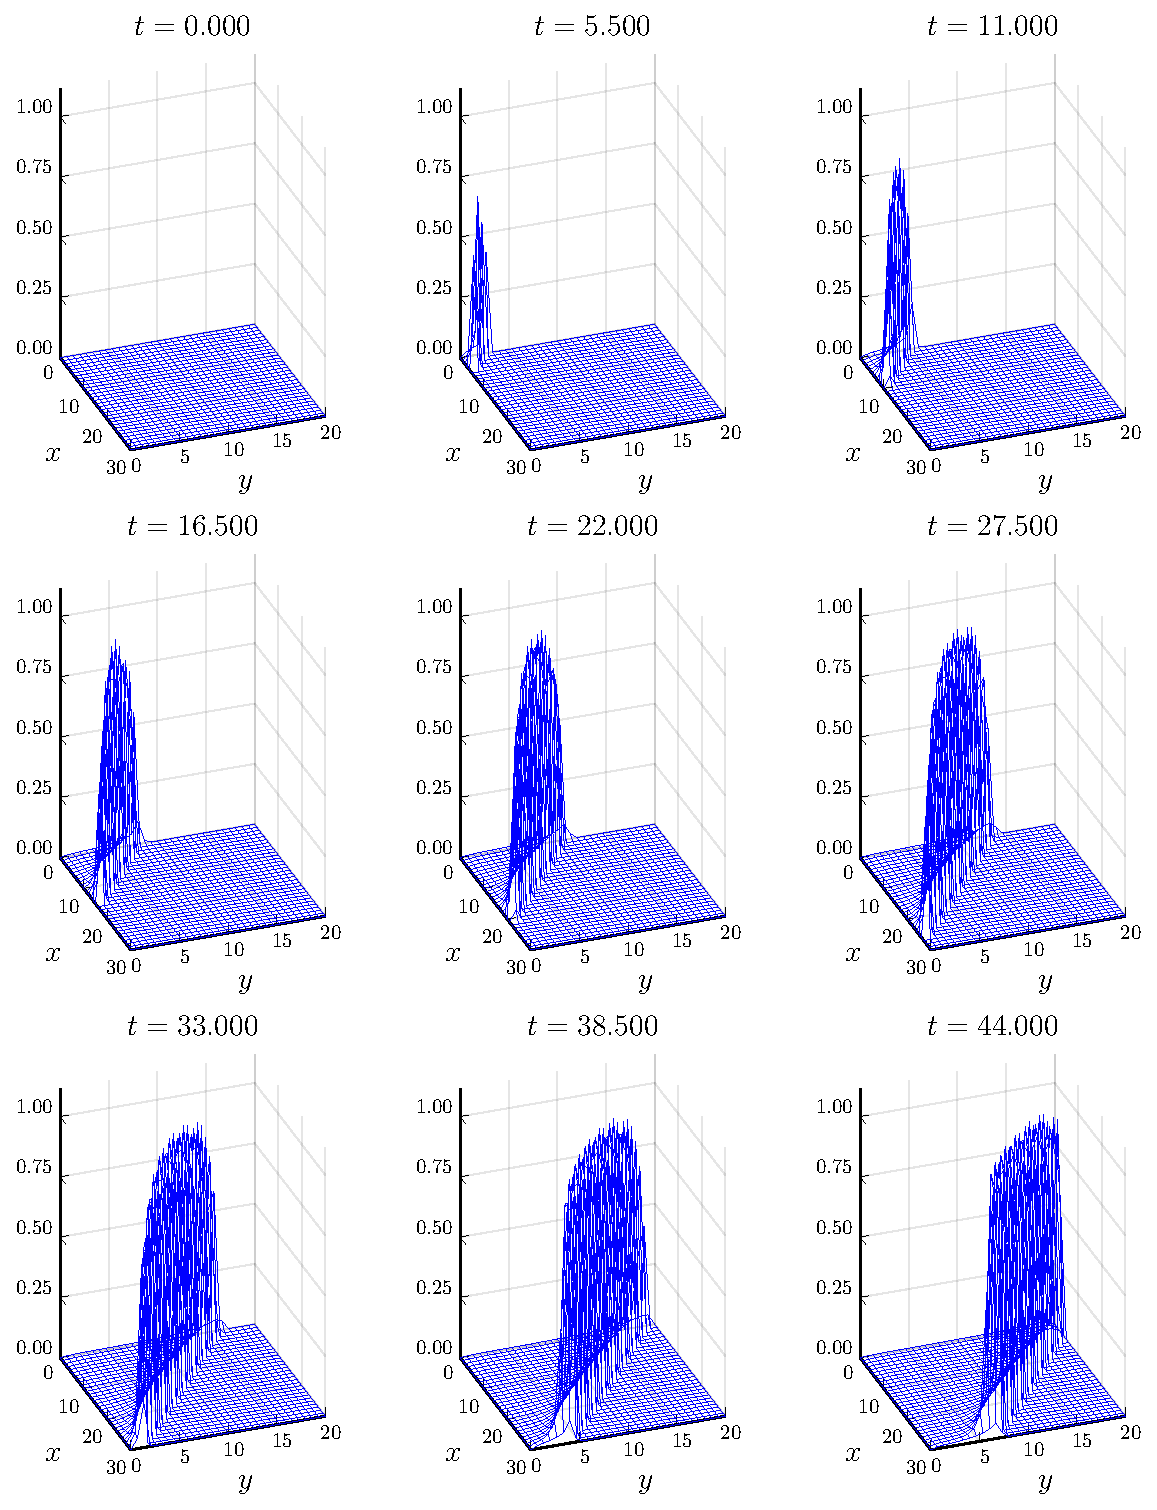
\includegraphics[width=\textwidth, keepaspectratio]{Разностные_схемы_на_статических_сетках/Программный_код_примеры_расчётов/explicit_scheme/problem_3_loc_err_wireframe.pdf}
    \caption{Серия графиков зависимости $|u(x, y, t) - u_h(x, y, t)|$ для фиксированных моментов времени $t \in [0, T]$.}
    \label{fig:problem_3_err}
\end{figure}
Работоспособность проверена на задаче, рассмотренной в статье \cite{самарский1963примеры}:
\begin{equation}\label{eq:problem_3}
    \textstyle
    \begin{cases}
        u_t = (4u^4 u_x)_x + \left( \frac{1}{4} u^2 u_y \right)_y, \quad (x, y, t) \in (0, 30) \times (0, 20) \times (0, 50)\\
        u(x, y, 0) = 0,\\
        u(0, y, t) = \mu_{-1}(y, t) = \begin{cases}
            \scriptstyle\frac{1}{2}\sqrt{-1 + \sqrt{1 + 16(t - 2y)}}, & t > 2y\\
            \hfill 0, & t < 2y
        \end{cases}\\
        u(30, y, t) = \mu_1(y, t) = \begin{cases}
            \scriptstyle\frac{1}{2}\sqrt{-1 + \sqrt{1 + 16(t - 30 - 2y)}}, & t > 30 + 2y\\
            \hfill 0, & t < 30 + 2y
        \end{cases}\\
        u(x, 0, t) = \mu_{-2}(x, t) = \begin{cases}
            \scriptstyle\frac{1}{2}\sqrt{-1 + \sqrt{1 + 16(t - x)}}, & t > x\\
            \hfill 0, & t < x
        \end{cases}\\
        u(x, 20, t) = \mu_2(x, t) = \begin{cases}
            \scriptstyle\frac{1}{2}\sqrt{-1 + \sqrt{1 + 16(t - x - 40)}}, & t > x + 40\\
            \hfill 0, & t < x + 40
        \end{cases}
    \end{cases}
\end{equation}
На \figref{fig:problem_3_wireframe} представлено численное решение задачи \eqref{eq:problem_3}.
Решение этой задачи также представляет собой вид бегущей волны с разрывом производных решения в точках фронта.
Было проведено сравнение с аналитическим решением:
\begin{equation*}
    u(x, y, t) = \begin{cases}
        \frac{1}{2}\sqrt{-1 + \sqrt{1 + 16(t - x - 2y)}}, & t \ge x + 2y\\
        0, & t < x + 2y
    \end{cases}
\end{equation*}
На \figref{fig:problem_3_err} отражена локальная погрешность решения.
Видно, что ситуация аналогична той, которая была описана выше для одномерного уравнения, а именно: погрешность в окрестности особых точек на порядки превышает погрешность в остальной области.
Число этих точек, по сравнению с общим числом точек сетки невилико, а именно, отношение 
$
    \frac{N_{\text{особ.}}}{N_{\text{общ.}}} \rightarrow 0
$
при
$
    N_{\text{общ.}} \rightarrow 0
$
Это утверждение прямо говорит о том, что просто измелчать равномерную сетку для достижения заданной точности в окрестности особых точек \emph{нецелесообразно}.